\documentclass{article}
\usepackage[utf8]{inputenc}
\usepackage[T1]{fontenc}
\usepackage[english]{babel}
\setlength{\parindent}{0pt}
\usepackage{hyperref}
\hypersetup{
    colorlinks=true,
    linkcolor=blue,
    filecolor=magenta,      
    urlcolor=cyan,
    pdftitle={Sharelatex Example}}
\usepackage{graphicx}
\graphicspath{ {./pic/} }

\usepackage{fourier,amssymb,microtype,amsmath,gensymb}
\newcommand{\R}{\mathbb{R}}
\usepackage{mdframed,caption,xcolor}
\usepackage{tikz,tkz-euclide}

\title{Questions and Answers}
\author{Xiaoguang Ling \\  \href{xiaoguang.ling@econ.uio.no}{xiaoguang.ling@econ.uio.no}}
\date{\today}

\begin{document}

\maketitle

\tableofcontents

\newpage
%%%%%%%%%%%%%%%%%%%%%%%%%%%%%%%%%%%%%%%%%%%%%%%%%%%%%%%%%%%%%%%%%%%%%%%%%%%%%%%%%%%%%%%%%%%%%%
\section{Seminar 1}

%***************************************************
\subsection{question 1.26}

Q: Should it be "equality" in Kuhn-Tucker condition equation (6): $p_1x_1 + p_2x_2 \le y$ (slides pp.16)?

\vspace{2mm}

A: You can argue it is "equality" for a well defined
classical utility function, since the solution is always
on the boundary(you can always spend the rest part of your
budget to imporve your utility).

But note that Kuhn-Tucker condition describes the most
general case for a value maximization problem. If the 
utility function is weired, for example, in Figure \ref{fig:ktc},
the utility function ($u(x_1,x_2) =3-\left(x_1-2\right)^2-\left(x_2-2\right)^2$) looks like a cone, the "peak" of the cone
is within the "budget plane($x+y=6$)". Your utility can therefore be maximized within your budget. "$\le$" allows this case.

\vspace{2mm}

{\centering
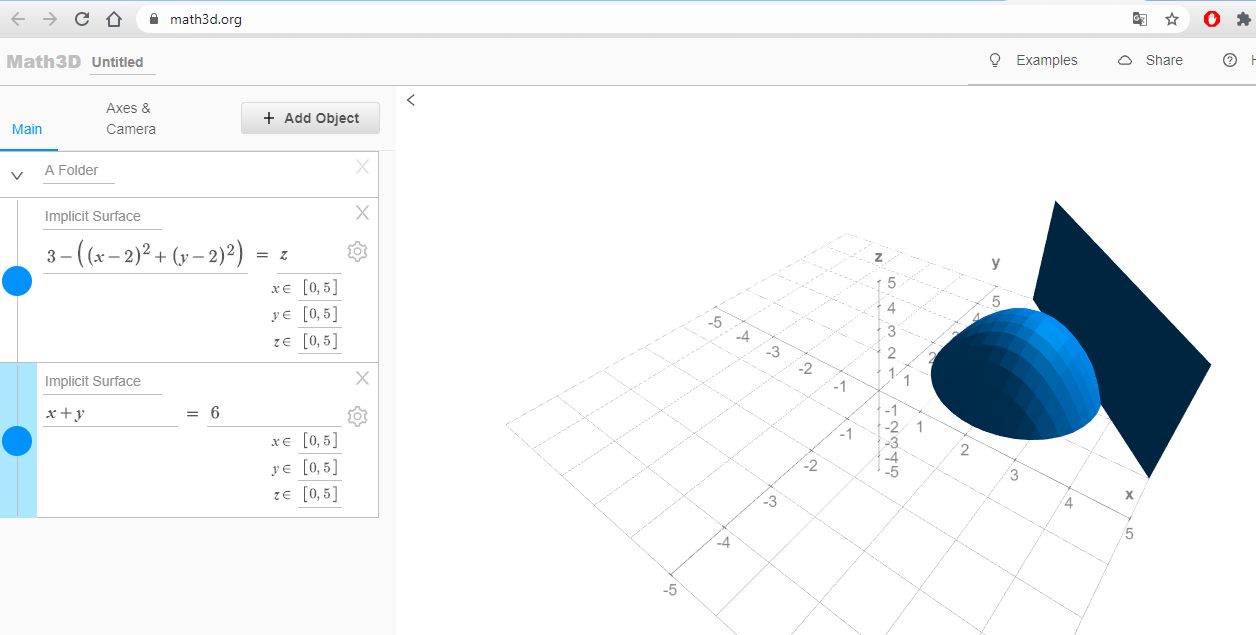
\includegraphics[width=1\textwidth]{1.q_ktc}
\captionof{figure}{A cone-like utility function and a loose budget}
\label{fig:ktc}}

\vspace{2mm}

Try to make some graphs yourself on \href{https://www.math3d.org/}{https://www.math3d.org/}. Always remember your utility is the 
extra dimension (z-axis in Figure \ref{fig:ktc}).


%%%%%%%%%%%%%%%%%%%%%%%%%%%%%%%%%%%%%%%%%%%%%%%%%%%%%%%%%%%%%%%%%%%%%%%%%%%%%%%%%%%%%%%%%%%%%%
\section{Seminar 2}
\subsection{Exercise 1.51 }
Q: In exercise 1.51 we are asked to compute the substitution term in the Slutsky equation. My question is about the derivation of $y$. I see that when we take the derivative of $y$ wrt $p_2$ we get zero. Isn't $7=p_1x_1 +p_2x_2$, so the derivative must be $x_2$?

\medskip

In the utility maximization problem, the consumer maximizes his/her utility restricted by the income $y$, some money that can be understood as a constant number.

\medskip

What the consumer will do, is to smartly choose $x_1$ and $x_2$, s.t. $x1 +x2 = y$, here the variables are $x_1$ and $x_2$, not $y$, while $y$ is a parameter.

\medskip

In other words, even though a smart consumer will choose $x_1 +x_2 = y, y$ is not what he/she can decide, it the income decided by his/her boss.

\medskip

When you take derivative of the Marshallian demands, $x(p,y)$, wrt $p$, you are asking, "given income $y$, what will happen to the optimal demand when price $p$ changes?"

%%%%%%%%%%%%%%%%%%%%%%%%%%%%%%%%%%%%%%%%%%%%%%%%%%%%%%%%%%%%%%%%%%%%%%%%%%%%%%%%%%%%%%%%%%%%%%
\section{Seminar 5}
\subsection{Textbook J\&R page 149. and page 11 in seminar 5 solution}

There is a typo in the textbook.

It should be $\Pi(p,w)$, since $x$ and $y$ are only those that can maximize $py -wx$ st. $y \le f(x)$. In other words, the $x$ and $y$ are $x^*$ and $y^*$. Then value function $P_i$ is only a function of $p,w$. 

\medskip

I copied it directly from the textbook so there is also a typo in my solution.
%%%%%%%%%%%%%%%%%%%%%%%%%%%%%%%%%%%%%%%%%%%%%%%%%%%%%%%%%%%%%%%%%%%%%%%%%%%%%%%%%%%%%%%%%%%%%%

\section{Previous exams -Econ 3220/4220}

%***********************************************************
\subsection{\href{https://www.uio.no/studier/emner/sv/oekonomi/ECON4220/previous-exams/econ32_4220_2019h_sensorveiledning.pdf}{Econ 3220/4220 Exam 2019}}


\subsubsection{Q2.d PBE}

(To make the guidelines more readable) The PBE are:
$\{DN', CE', p=1,q=0\}$ and $\{NN', EE', p<2/3, q=1/2\}$. 

\smallskip

Be careful that in this question, $I$ is player $2$ and $U$ is player $1$.

\smallskip

For the separating one, if player $2$ (i.e. $I$) deviates from $D$ to $N$, when player $1$ (i.e. $U$) observes $N$, he/she will think it's Type $L$, according to the updated belief. 
"Facing with a (fake) Type $L$ individual", the BR of player $1$ (i.e. $U$)  is to choose $E'$. 

\smallskip

The payoff is $(0,0)$. Therefore player $2$ will not deviate.




%***********************************************************
\subsection{\href{https://www.uio.no/studier/emner/sv/oekonomi/ECON4220/previous-exams/econ32_4220_2019h_postponed_guidelines.pdf}{Econ 3220/4220 Postponed exam 2019}}

\subsubsection{Q1.a Anastasia}
Q: Isn't $\alpha$ the measure of preference?

\medskip

Yes, $\alpha$ measures the relative importance of $x_1$ and $x_2$. 
In this question, since $x_1$ and $x_2$ are demands in the 2 periods, they can be understood as the same good but one in today, and one in the future. 
Therefore the preference to $x_1$ and $x_2$ is related to how you value the commodity in today and tomorrow. That's why the solution said it's related to the discount factor.


\subsubsection{Q1.b Anastasia}
\textbf{Q: What is the Budget constraint in these cases?}

\medskip
 (There is a typo in task 1: it should be $x_i$ instead of $x_1$)

\medskip

the constraint contains 2 periods.

\begin{itemize}
\item In period 1, assume the consumer decides to save $s$, and the total monetary endowment is $m$, then the constraint is $w_1 x_1 + s = m$;

\item In period 2, the save brings some return $r \times s$, together with the capital $s$, the total income should be $(1+r)s$. Therefore the constraint is $w_2x_2 = (1+r)s$. 
\end{itemize}

Combining the two constraint gives $w_1 x_1 + \frac{w_2}{1+r} x_2 = m$. This is the constraint you should use in Lagrangian.

\medskip

\textbf{About the guidelines}

\medskip

I found that the guidelines must make additional assumptions:

\medskip

Firstly, the $r$ in the guideline is the "$1+r$" I mentioned. It's just a notation difference. So here we assume saving $s$ becomes $rs$ in period 2.

\smallskip

Secondly, it must assume $w_1=w_2=1$. It's reasonable since $x_1$ and $x_2$ are "demand in period 1 and 2", if we assume there is no inflation (no price change in the two periods), then $w_1=w_2$. Assuming $w_1=w_2=1$ will simplify the calculation.

\smallskip

Then the budget constraint becomes $$x_1 + \frac{1}{r}x_2=m$$
(It looks the same as the budget constraint when the price of $x_1$ is $1$ and the price of $x_2$ is $\frac{1}{r}$).

\smallskip

Solving the Lagrangian gives,

$$x_1 = \alpha m$$
$$x_2 = (1-\alpha) m r$$

\textcolor{red}{Somehow $x_2$ is still different from the guidelines... Remind me if I made any mistake!}

\smallskip

My solution satisfies Roy's identity too if you understand $\frac{1}{r}$ as the price of $x_2$ according to the budget constraint.

\medskip

Denote $\frac{1}{r}$ as $w_2' $, then $r = \frac{1}{w_2'} \Rightarrow x_2 = (1-\alpha) m r = (1-\alpha) m \frac{1}{w_2'}$. Thus,

$$\frac{\partial V/ \partial w_2'}{\partial V/ \partial m}= (1-\alpha) m \frac{1}{w_2'} =(1-\alpha) m r = x_2$$


\subsubsection{Q2. BoltNa}

It seems the guidelines assumed $\alpha =1$, then you'll get $1/2$ in part 2a; similarly, in 2b, if you keep $\alpha$ as an parameter, the cost function is (the calculation is standard Lagrangian method but may seem messy, so be patient!)
$$C = [w_1 \alpha + w_2 + 2 (w_1 w_2 \alpha)^{1/2}] y$$
When $\alpha=1$,
$$C = [w_1 + w_2 + 2 (w_1 w_2 )^{1/2}] y = (\sqrt{w_1}+\sqrt{w_2})^2 y$$


%################################################################################
\section{Previous exams -Econ 3200/4200}
%***********************************************************
\subsection{\href{https://www.uio.no/studier/emner/sv/oekonomi/ECON3200/previous-exams/ECON3200_4200-2015H.pdf}{Fall 2015}}
\subsubsection{Q1. A.MRTS}

The solution used a different notation. In exam we should use the notation used in our textbook and seminars, that is, $MRTS_{ij}$ means marginal rate of substitution of good $j$ for good $i$.

\medskip

It means how much $j$ you're willing to give up to increase one unit $i$. So in this question, $MRTS_{12}= \frac{1}{2} \frac{z_2}{z_1}$.


%***********************************************************
\subsection{\href{https://www.uio.no/studier/emner/sv/oekonomi/ECON3200/previous-exams/econ32_4200-2017h-sensorveiledning.pdf}{Fall 2017}}

\subsubsection{Q8. Dominance}

\begin{center}
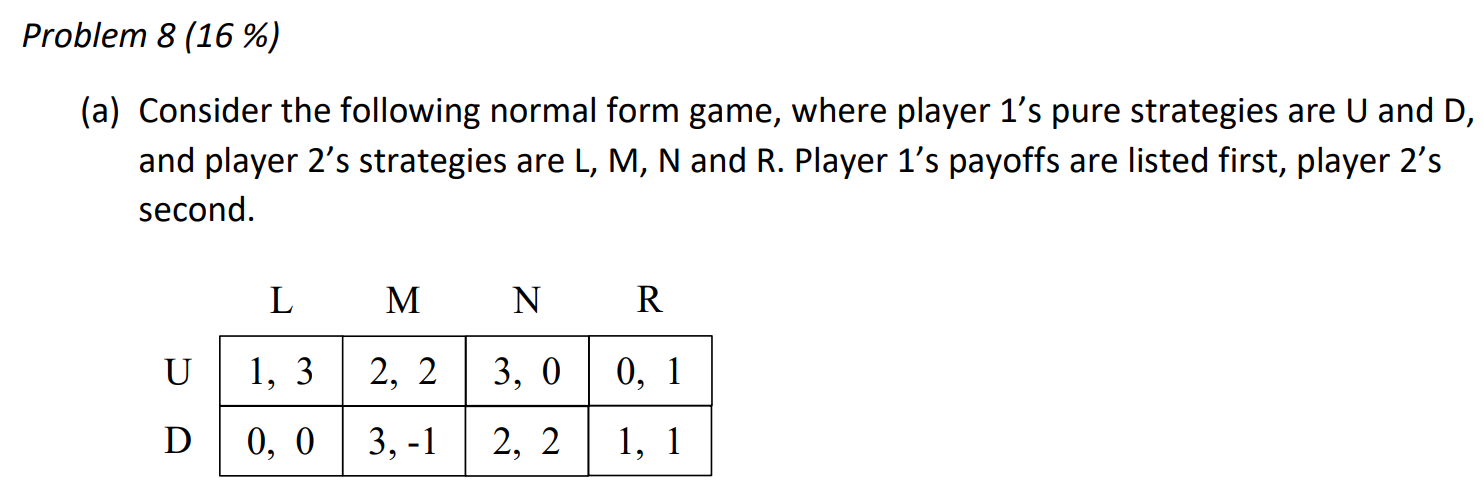
\includegraphics[width=0.8\textwidth]{e3200_2017_q8}
\end{center}
\vspace{2mm}

For player 2, $R$ is actually dominated by the mixed strategy of $L$ and $N$. For example, by mixing $L$ and $N$ with probability $(0.4,0,6)$, the expected payoff for player 2 is $1.2$ and $1.2$ after $U$ and $D$, higher than R (payoff 1 and 1 after $U$ and $D$).

\smallskip

Note that the definition of dominance applies to both pure and mixed strategies since they are both based on some belief. 
(See also Watson pp.50).  By iterated dominance method, we can always cross a strategy out as long as it's dominated by other (either pure or mixed) strategies. 

\smallskip

After we remove $M$ and $R$, we can easily find $U$ dominates $D$, and $L$ dominates $N$. The only rationalizable strategy is $U$ for player 1 and $L$ for player 2. The only NE is $(U,L)$


%***********************************************************
\subsection{\href{https://www.uio.no/studier/emner/sv/oekonomi/ECON3200/previous-exams/econ32_4200-2018h.pdf}{Fall 2018}}

\subsubsection{Q1.  Cost function}

It seems that the question itself omitted many prerequisites such as the how the production function looks like (continuous and strictly increasing, as assumed in our textbook pp.138).

\medskip

Since if we take these prerequisites into consideration, none of the arguments is correct, the question must take those assumptions as granted... Here is how I think about them one by one:

\medskip

(If $f$ is continuous and strictly increasing)
\begin{enumerate}
\item True. If f is also strictly quasi-concave, the derivative of the cost function with respect to input price gives the compensated demand of that input (it's called conditional input demand in our textbook, though)
\item True. For $w \gg 0$, c is strictly increasing in $y$, therefore must also be nondecreasing in y
\item False. It should be increasing, not decreasing in $y$
\item True. It's increasing in w, and strictly increasing in at least one ($w_i$). This is a conclusion in the old textbook for econ4200
\item False. It's concave in input prices w, not necessarily in $y$. 
\item False. Degree 1.
\item False. The same as argument 4. It's increasing in $w$, not necessary to be strict.
\item True. Same as 4. and 7.
\end{enumerate}

\subsubsection{Q3. Uncertainty}

\begin{center}
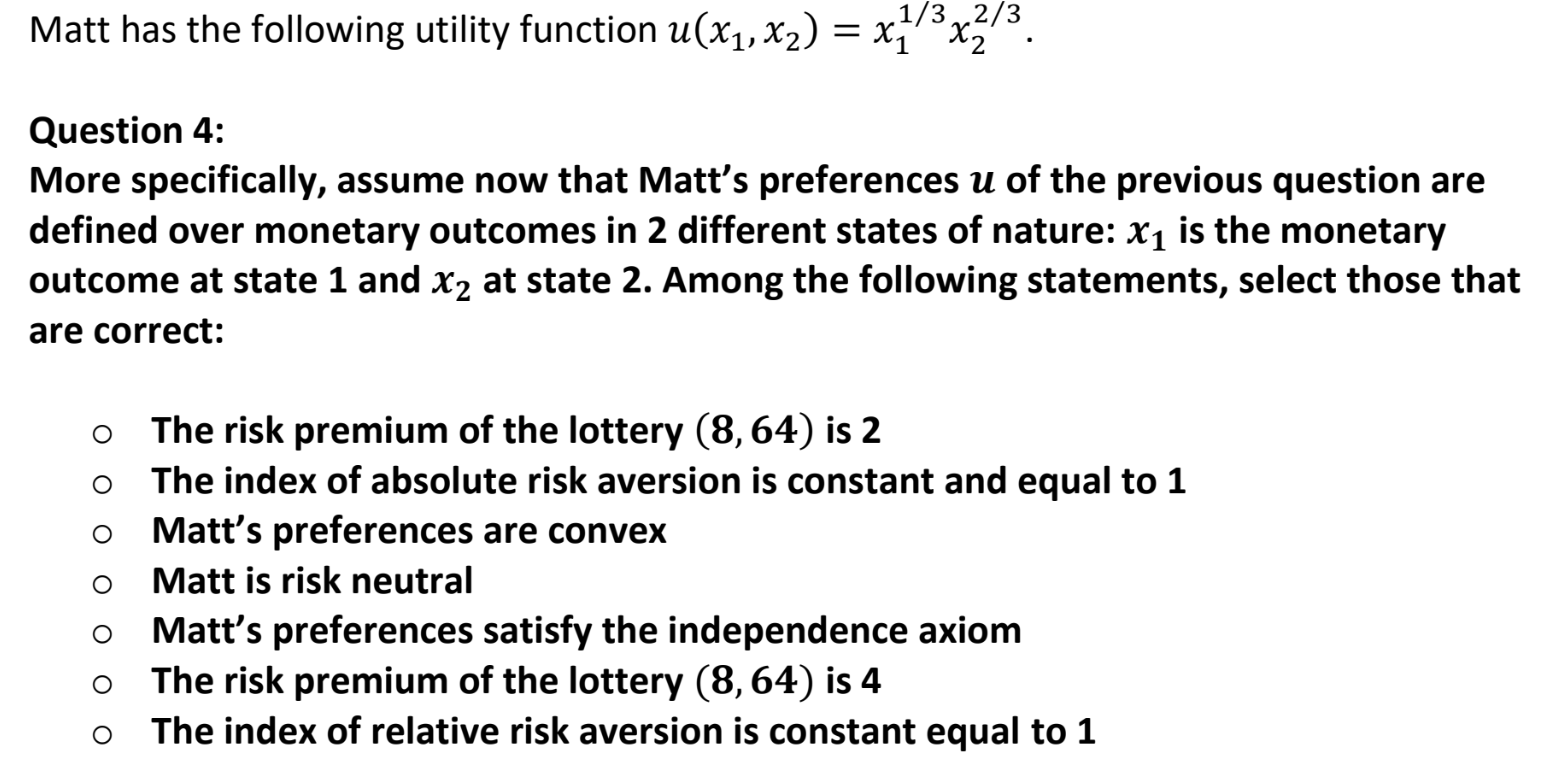
\includegraphics[width=0.8\textwidth]{e3200_2018_q3}
\end{center}
\vspace{2mm}

We should monotonically transform the utility function  $x_1^{\frac{1}{3}}{x_2}^{\frac{2}{3}}$ into the form that looks like an expectation, i.e. $(\frac{1}{3})ln x_1 + (\frac{2}{3})ln x_2$. Then the probability must be $(\frac{1}{3},\frac{2}{3})$ for the two states. 

\smallskip

The lottery $(8,64)$ means that $x_1$ value is $8$, and $x_2$ value is 64. The expected utility of the lottery is:

$$E(u)= \frac{1}{3} ln8 +\frac{2}{3} ln64 = 5ln2 = ln32$$

Denote certainty equivalent as CE,
$$ln(CE)=ln32 \Rightarrow CE = 32$$

Denote the monetary outcome as $m$, then
$$E(m) = (\frac{1}{3}) \times 8 +  (\frac{2}{3}) \times 64 = \frac{136}{3}$$

The risk premium is $$E(m)-CE = \frac{136}{3} -32$$

It seems both of the two options regarding risk premium are wrong, weird value though...

\medskip

When calculating the risk aversion, we use the original utility function (which is called "cardinal" utility function sometimes, here it is $lnx$) instead of the expected utility or the one before monotonic transformation. 

\smallskip

Therefore there is only one variable x and the first derivative is $1/x$. The risk aversion is caused by the fact that lnx is concave towards the x-axis.

\medskip

In the end, only the following 2 statements are true:

\begin{itemize}
\item Matt's preferences satisfy the independence axiom
\item The index of \textbf{relative} risk aversion is constant equal
to 1
\end{itemize}

Independence axiom is not well explain in our textbook. You can find the definition \href{https://www.uio.no/studier/emner/sv/oekonomi/ECON4260/h17/dokumenter/exputil.pdf}{here}.


%***********************************************************
\subsection{\href{https://www.uio.no/studier/emner/sv/oekonomi/ECON3200/previous-exams/econ32_4200-2019v-sensorveiledning.pdf}{Spring 2019}}

Q: The competitive firm FF has a production function of the form:
$F = 2L + 5K$, where $L$ denotes labor and $K$ capital. Assume salary $w=2$ and capital cost is $r=4$. What is the minimal cost of producing 10 units of output?


\bigskip
A: You can solve it in the following 3 ways:

\medskip

\textbf{1. Kuhn Tucker condition (not recommended)}

In this question, you're going to solve the cost minimization problem: $\min 2L + 4K , s.t. \  f(x) > = 10, L\ge0, K\ge0$. \\
You can definitely use Kuhn Tucker condition to solve it, similar to the question in our seminar 1, since the object function is also linear. 

\bigskip

\textbf{2. Substitute the constraint into the object function (be careful with the domain)}

Since you're going to minimize the cost, it's not reasonable to produce more than required (i.e. $10$, because cost function is increasing in output y), you will let $f(x)=10$, i.e. $F= 2L+5K=10$, or $2L=10-5K$.​ This relation holds as long as you want to minimize the cost. 
\medskip

Also, don't forget you have  $L\ge0$ and $K\ge0$.  Thus $2L=10-5K$ must also be non-negative, we have $10-5K \ge0, K\le2$. The domain of $K$ is $[0,2]$ \\
You can now substitute $2L=10-5K$ into your object function, $2L+4K$, and your minimization problem​ becomes $\min 10-5K +4K$ , or $\min 10 - K$. The object function is decreasing in K,  you want K to be as great as possible in its domain $[0,2]$, to minimize the cost. \\
So you choose $K=2, L=0$, minimized cost is $8$.
\medskip

In exam, you can write it concisely:
\medskip

 $\min 2L + 4K \  s.t. \  f(x) > = 10, L\ge0, K\ge0$ \\
Since cost function is increasing in output, $f(x)=10, i.e. \  F= 2L+5K=10$. Therefore: $2L=10-5K$.  Objection function becomes: 10-5K+4K=10-K, decreasing in K. \\
Besides, $K\ge0,  L\ge0$ and $2L=10-5K$  lead to $K \in [0,2]$. \\
Therefore $K^*=2, L^*=0$, 

\bigskip

\textbf{3. Cheapest per unit of product (recommended)}

Since the production function shows perfect substitution between $L$ and $K$, the firm chooses only the cheapest per unit of product input. Recall that perfect substitution means $K$ and $L$ are the same thing, just with different package, in the view of the firm.

\medskip
To produce $1$ unit output, according to $F = 2L+5K$, you need either $0.5$ unit $L$ or $0.2$ unit $K$. The price for $0.5$ unit $L$ is $0.5 \times 2 =1$; the price for $0.2$ unit $K​$ is $0.2 \times 4 =0.8$.
For $1$ unit output, $K$ is the cheapest input. Therefore the firm chooses $L=0, F=5K$. When $F=10$, $K=2$, the cost is $2 \times 4 =8$.


\end{document}
